\documentclass[a4paper,oneside,12pt,DIV=12,titlepage]{scrartcl}

%Typography
\usepackage{fontspec}
\setromanfont{STIX Two Text}
\setsansfont{Source Sans Pro}
\setmonofont{PT Mono}

\usepackage{microtype}

%Localization
\usepackage{polyglossia}
\setdefaultlanguage{ukrainian}
\PolyglossiaSetup{ukrainian}{indentfirst=true}

%Math typesetting
\usepackage{amsmath}
\usepackage{unicode-math}
\setmathfont{STIX Two Math}

%Table typesetting
\usepackage{booktabs}

%Including graphics
\usepackage{graphicx}

\usepackage{subcaption} % side-by-side figures

%Drawing electrical circuits
\usepackage{circuitikz}

%Itemize separator
\def\labelitemi{—}

\begin{document}
	\begin{titlepage}
		\begin{center}
			Міністерство освіти і науки України\\
			Національний авіаційний університет\\
			Навчально-науковий Інститут\\
			Комп'ютерних інформаційних технологій\\
			Кафедра комп'ютеризованих систем управління
			
			\vspace{\fill}
				Лабораторна робота №2\\
				з дисципліни «Комп'ютерна електроніка»\\
				на тему: «Дослідження біполярного транзистора»\\
				Варіант №
				
			\vspace{\fill}
			
			\begin{flushright}
				Виконав:\\
				студент ННІКІТ СП-225\\
				Клокун Владислав\\
				Перевірив:\\
				Андрєєв О.В.
			\end{flushright}
			Київ 2017
		\end{center}
	\end{titlepage}
	
	\tableofcontents
	\newpage
	
	\section{Мета та основні завдання роботи}
		\begin{enumerate}
			\item Ознайомитись з принципом дії, схемами ввімкнення і ВАХ біполярного транзистора.
			\item Набути практичних навичок у побудові вольт-амперних характеристик біполярного тразистора.
			\item Вивчити схеми ввімкнення біполярних транзисторів і їхні вольт-амперні характеристики.
			\item Освоїти методику побудови за вхідною напругою інших струмів і напруг біполярного транзистора.
		\end{enumerate}
	
	\section{Короткі теоретичні відомості}
		\subsection{Біполярний транзистор і його структура}
			Біполярним транзистором називається напівпровідниковий прилад із двома взаємодіючими \textit{p-n}-переходами, підсильвальні властивості якого засновані на явищах інжекції й екстракції.
			
			Біполярний транзистор складається з трьох напівпровідникових шарів з чергуючимся типом примісної провідності: емітера, бази та колектора. В залежності від порядку їх слідування розрізняють \textit{n-p-n}- та \textit{p-n-p}-транзистори.
			
		\subsection{Умовно-графічні зображення біполярних транзисторів}
			На рисунках зображені умовно-графічні позначечння біполярних транзисторів \emph{p-n-p}- і \emph{n-p-n}-типу.
			
			\begin{figure}[h]
				\begin{subfigure}[b]{0.45\textwidth}
					\centering
					\begin{circuitikz}
						\draw (0,0) node[pnp](pnp){};
						\draw (pnp.E) node[above]{Е};
						\draw (pnp.C) node[below]{К};
						\draw (pnp.B) node[left]{Б};
					\end{circuitikz}
					\caption{Транзистор p-n-p-типу}
				\end{subfigure}
				\quad
				\begin{subfigure}[b]{0.45\textwidth}
					\centering
					\begin{circuitikz}
						\draw (0,0) node[npn](npn){};
						\draw (npn.E) node[below]{Е};
						\draw (npn.C) node[above]{К};
						\draw (npn.B) node[left]{Б};
					\end{circuitikz}
					\caption{Транзистор n-p-n-типу}
				\end{subfigure}
				\caption{Умовно-графічні позначення транзисторів}
			\end{figure}
			
		\subsection{Схеми ввімкнення біполярного транзистора}
			Біполярний транизстор має три схеми ввімкнення: із загальною базою, загальним емітером і загальним колектором. В обчислювальній техніці найбільш поширена схема з загальним емітером, оскільки при такому підключенні коефіціент підсилення максимальний:  $\beta \gg 1$.
			
			Також існує інверсне підключення транзистора, коли емітер і колектор міняються функціями. При такому підключенні для позначення параметрів використовують індекс $I$: $\alpha_I$, $\beta_I$ тощо.
		
		\subsection{Вхідна і вихідна вольт-амперна характеристика біполярного транзистора}
			Біполярні транзистори мають чотири статичні вольт-амперні характеристики:
				\begin{enumerate}
					\item Вхідні: зв'язують струм і напругу на вході транзистора.
					\item Вихідні: зв'язують струм і напругу на виході транзистора.
					\item Характеристики передачі: зв'язують струми чи напруги на виході зі струмами чи напругами на вході.
					\item Характеристики зворотнього зв'язку: зв'язують напруги чи струми на вході зі струмами чи напругами на виході.
				\end{enumerate}
		
		\subsection{Навантажувальна пряма}
			Навантажувальна пряма --- це пряма, що однозначно пов'язує струм і напругу на виході, та є траекторією руху робочої точки в посилюючому режимі роботи біполярного транзистора, тобто при включенні в ланцюг навантажувального резистора $R_{\textnormal{К}}$. Ця пряма описується рівнянням:
			\begin{equation}
				I_{\textnormal{К}} = \frac{E_\textnormal{K} - U_{\textnormal{КЕ}}}{R_\textnormal{K}} = \frac{E_{\textnormal{K}}}{R_{\textnormal{K}}} - \frac{U_{\textnormal{КЕ}}}{R_{\textnormal{K}}},
				\label{eq:ik}
			\end{equation}
			де $I_{\textnormal{К}}$ --- вихідний струм, $E_{\textnormal{К}}$ --- електрорушійна сила джерела живлення, $U_{\textnormal{КЕ}}$ --- напруга «колектор-емітер», $R_{\textnormal{К}}$ --- опір резистора навантаження.
			
			З формули \ref{eq:ik} видно, що при $I_{\textnormal{К}} = 0$, $U_{\textnormal{КЕ}} = E_{\textnormal{К}}$. Для знаходження першої точки навантажувальної прямої --- точки $K$ --- необхідно відкласти на осі абсцис величину $E_{\textnormal{К}}$. У цій точці тразистор замкнений. Для знаходження другої точки навантажувальної прямої --- точки $B$ --- використаємо величину $U_{\textnormal{КЕ}}$ таким чином: припустимо, що $U_{\textnormal{КЕ}} = 0$, тоді $I_{\textnormal{К}} = \frac{E_{\textnormal{К}}}{R_{\textnormal{К}}}$. Пряма $BK$ і буде шуканою навантажувальною прямою.
			
		\subsection{$h$-параметри}
			Величини, що зв'язують малі збільшення струмів і напруг називаються диференціальними параметрами транзисторів. Для транзисторів запропоновано багато систем параметрів, однак, основними вважаються змішані (\emph{hybrid}) параметри, які позначають літерою \emph{h}.
			
			У системі h-параметрів за незалежні змінні обирають вхідний струм $I_1$ і напругу $U_2$, а за залежні --- вхідну напругу $U_1$ і вихідний струм $I_2$. Це пов'язано з малим вхідним і великим вихідним опорами транзистора. Для схеми ввімкнення із загальним емітером це такі величини:
				\begin{itemize}
					\item вхідний струм $I_{\textnormal{Б}}$ і напруга $U_{\textnormal{БЕ}}$.
					\item вихідний струм $I_{\textnormal{К}}$ і напруга $U_{\textnormal{КЕ}}$.
				\end{itemize}
				
				Тоді система рівнянь, що пов'язує h-параметри має такий вигляд:
				\begin{equation}
					\begin{cases}
						U_{\textnormal{БЕ}} = h_{11} I_{\textnormal{Б}} + h_{12} U_{\textnormal{КЕ}}\\
						I_{\textnormal{К}} = h_{21} I_{\textnormal{Б}} + h_{22} U_{\textnormal{КЕ}}\\
					\end{cases}
					\label{eq:hparamsys}
				\end{equation}
			
			Із системи рівнянь \ref{eq:hparamsys} випливає фізичний зміст і найменування \emph{h}-параметрів. Вхідний опір транзистора при короткому замиканні на виході для змінної складової струму:
				\[
					h_{11} = \frac{U_1}{I_1}, \, U_2 = 0.
				\]
			
			Коефіцієнт зворотного зв'язку за напругою при розімкнутому вході для змінної складової струму:
				\[
					h_{12} = \frac{U_1}{U_2}, \, I_1 = 0.
				\]
				
			Диференціальний коефіцієнт передачі струму:
				\[
					h_{21} = \frac{I_2}{I_1}, \, U_2 = 0.
				\]
				
			Вихідна провідність транзистора при розімкнутому вході для змінної складової струму:
				\[
					h_{22} = \frac{I_2}{U_2}, \, I_1 = 0.
				\]
				
			Для визначення h-параметрів можна використовувати графоаналітичний спосіб, який, однак, має невисоку точність. Для цього на вхідних і вихідних характеристиках навколо робочої точки необхідно побудувати трикутники. На сім'ї взідних характеристик у робочій точці $A$ будують трикутник $ABC$. З точки $A$ проводять прямі, вінобіжні осі абсцис і осі ординат до перетинання з другою характеристикою в точках $B$ і $C$. З отриманого характеристичного трикутника знаходять всі необхідні величини для обчислення $h_{\textnormal{11Е}}$, $h_{\textnormal{12Е}}$. Відрізок $AB$ є $\Delta U_{\textnormal{БЕ}}$, а $AC$ --- збільшення $\Delta I_{\textnormal{Б}}$.
			
			Збільшення напруги колектора визначається як різниця напруг, при яких знімалися характеристики:
			\[
				\Delta U_{\textnormal{КЕ}} = U''_{\textnormal{КЕ}} - U'_{\textnormal{КЕ}}.
			\]
			
			Тоді:
			\[
				h_{\textnormal{11Е}} = \frac{\Delta U_{\textnormal{БЕ}}}{\Delta I_{\textnormal{Б}}} = \frac{AB}{AC};
			\]
			\[
				h_{\textnormal{12Е}} = \frac{\Delta U_{\textnormal{БЕ}}}{\Delta U_{\textnormal{КЕ}}} = \frac{AB}{U''_{\textnormal{КЕ}} - U'_{\textnormal{КЕ}}};
			\]
			
			У робочій точці $A'$ за вихідними характеристиками можна визначити параметри $h_{\textnormal{21Е}}$ і $h_{\textnormal{22Е}}$. Проводячи з точки $A'$ вертикальну пряму до перетинання з наступною характеристикою (точка $D'$), знаходимо збільшення струму колектора $\Delta I_{\textnormal{К}}$ при $U'_{\textnormal{КЕ}} = \mathrm{const}$. Відрізок $A'D'$ показує на збільшення струму бази $\Delta I_{\textnormal{Б}} = I_{\textnormal{Б5}} - I_{\textnormal{Б4}}$.
			
			Тоді:
			\[
				h_{\textnormal{21Е}} = \frac{\Delta I_{\textnormal{К}}}{\Delta I_{\textnormal{Б}}} = \frac{A'D'}{I_{\textnormal{Б5}} - I_{\textnormal{Б4}}}.
			\]
			
			Для визначення параметра $h_{\textnormal{22Е}}$ з точки $A'$ проводять пряму, рівнобіжну осі абсцис, необхідної довжини для виміру збільшення струму $\Delta I'_{\textnormal{К}} = B'C'$. За точками визначимо збільшення напруги колектора $\Delta U'_{\textnormal{БЕ}}$. Тоді:
			\[
				h_{\textnormal{22Е}} = \frac{\Delta I'_{\textnormal{К}}}{\Delta U'_{\textnormal{БЕ}}} = \frac{B'C'}{A'B'}.
			\]
			
			На рис. \ref{fig:VACs} зображені вольт-амперні характеристики біполярного транзистора з графоаналітичним методом пошуку навантажувальної прямої та h-параметрів.
			
			\begin{figure}[h]
				\centering
				\begin{subfigure}[b]{0.45\textwidth}
					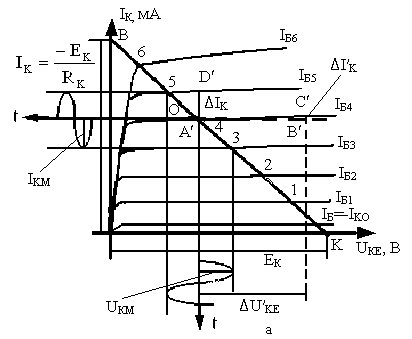
\includegraphics[width=\textwidth]{VAC-01.png}
					\caption{Вхідна ВАХ з навантажувальною прямою}
				\end{subfigure}
				\begin{subfigure}[b]{0.45\textwidth}
					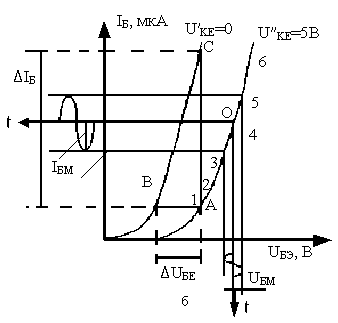
\includegraphics[width=\textwidth]{VAC-02.png}
					\caption{Вихідна ВАХ з відрізками для визначення $h_{11}$, $h_{12}$}
				\end{subfigure}
				\caption{Вольт-амперні характеристики біполярного транзистора}
				\label{fig:VACs}
			\end{figure}
			
	\section{Принципова схема віртуальних лабораторних установок}
		На рис. \ref{fig:scheme} зображена принципова схема віртуальної лабораторної установки для дослідження біполярного транзистора.
		
		\begin{figure}[h!]
			\centering
			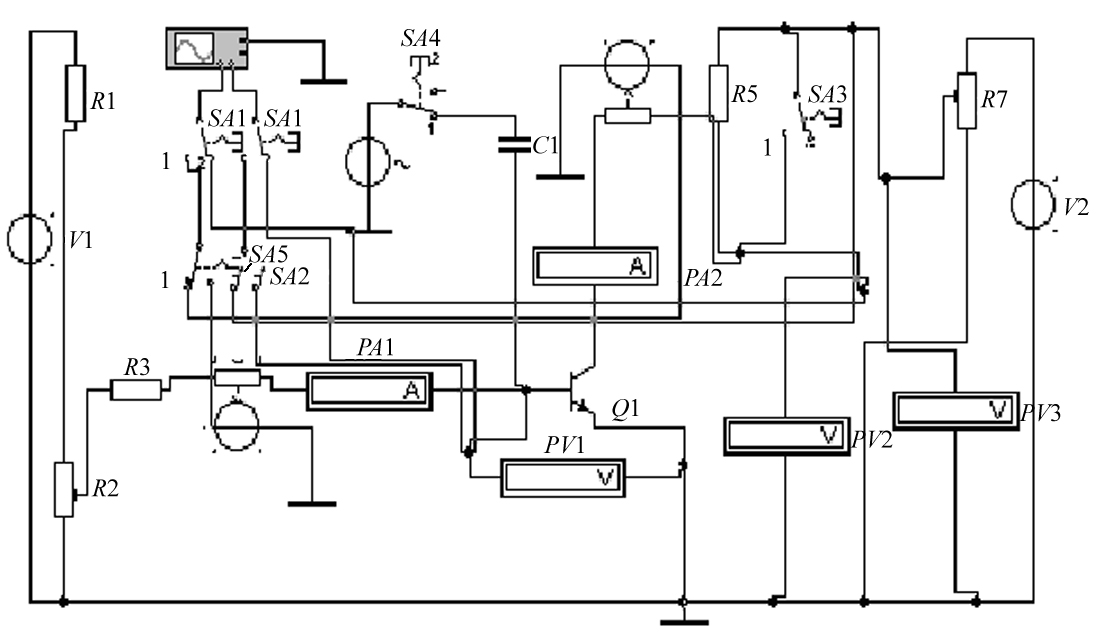
\includegraphics[width=\textwidth]{schematic-01.jpg}
			\caption{Принципова електрична схема віртуальної лабораторної установки}
			\label{fig:scheme}
		\end{figure}
		
	\section{Хід виконання завдання лабораторної роботи.}
		\subsection{Побудова вхідних вольт-амперних характеристик}
			\subsubsection{Підготовка лабораторної установки до роботи}
				Переводимо перемикачі у необхідні положення, вмикаємо та налаштовуємо осцилограф. Встановлюємо необхідну напругу за допомогою потенціометра $R_7$.
			
			\subsubsection{Увімкнення лабораторної установки}
				Вмикаємо лабораторну установку на моделювання за допомогою відповідної кнопки графічного інтерфейсу.
				
			\subsubsection{Побудова першої вольт-амперної характеристики}
				За допомогою осцилографа отримуємо першу вхідну вольт-амперну характеристику, зображену на рис. \ref{fig:graph001}.
				
				\begin{figure}[h]
					\centering
					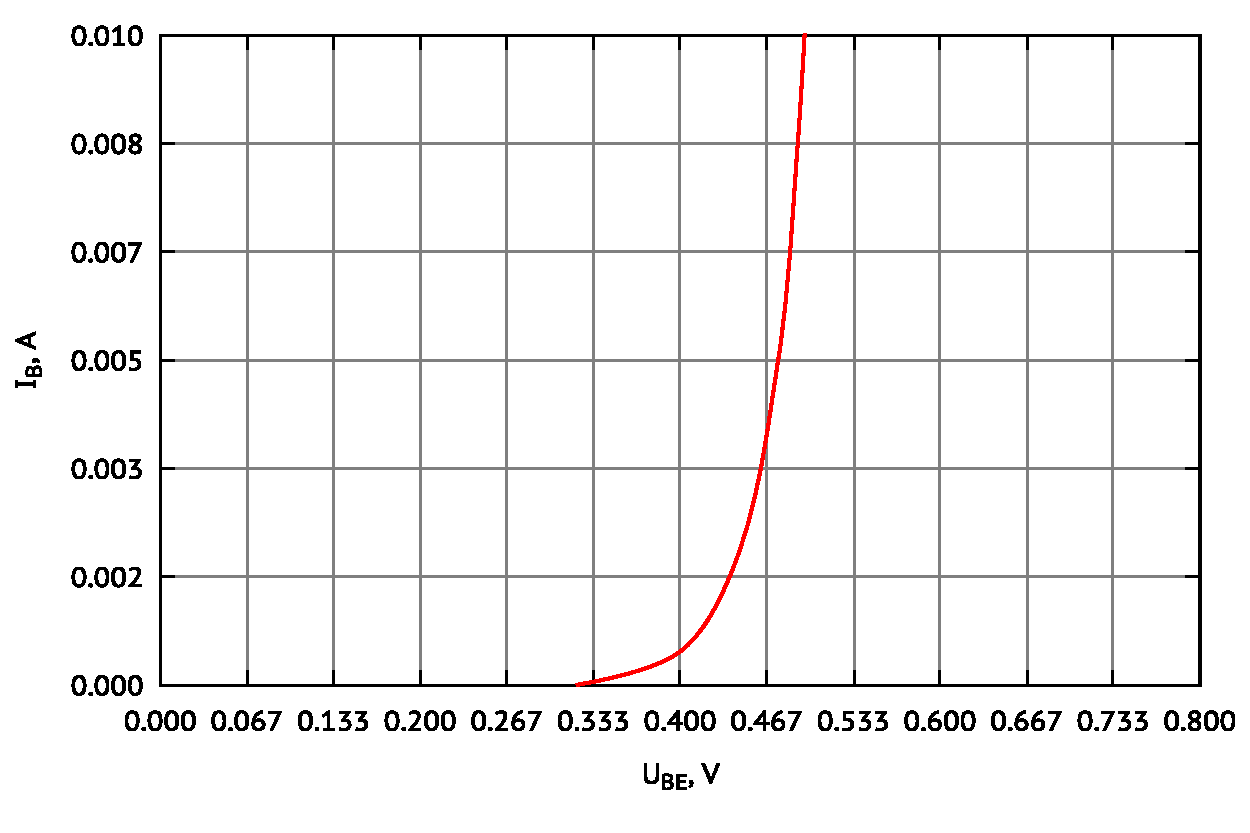
\includegraphics[width=0.45\textheight]{graph001-0.pdf}
					\caption{Перша отримана вхідна вольт-амперна характеристика}
					\label{fig:graph001}
				\end{figure}
				
			\subsubsection{Побудова другої вольт-амперної характеристики}
				За допомогою осцилографа отримуємо другу вхідну вольт-амперну характеристику, зображену на рис. \ref{fig:graph002}.
				
				\begin{figure}[h]
					\centering
					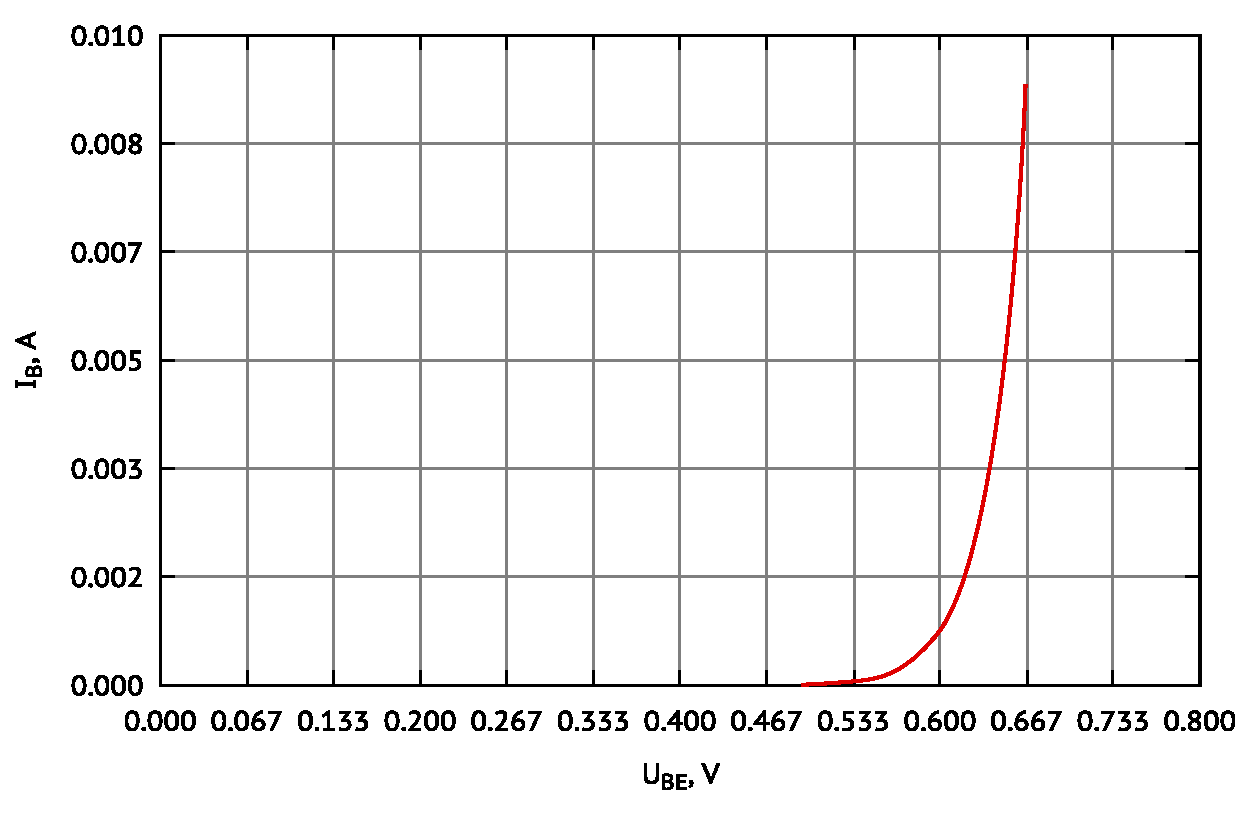
\includegraphics[width=0.45\textheight]{graph002-0.pdf}
					\caption{Друга отримана вхідна вольт-амперна характеристика}
					\label{fig:graph002}
				\end{figure}
				
			\subsubsection{Побудова третьої вольт-амперної характеристики}
				За допомогою осцилографа отримуємо третю вхідну вольт-амперну характеристику, зображену на рис. \ref{fig:graph003}.
				
				\begin{figure}[h]
					\centering
					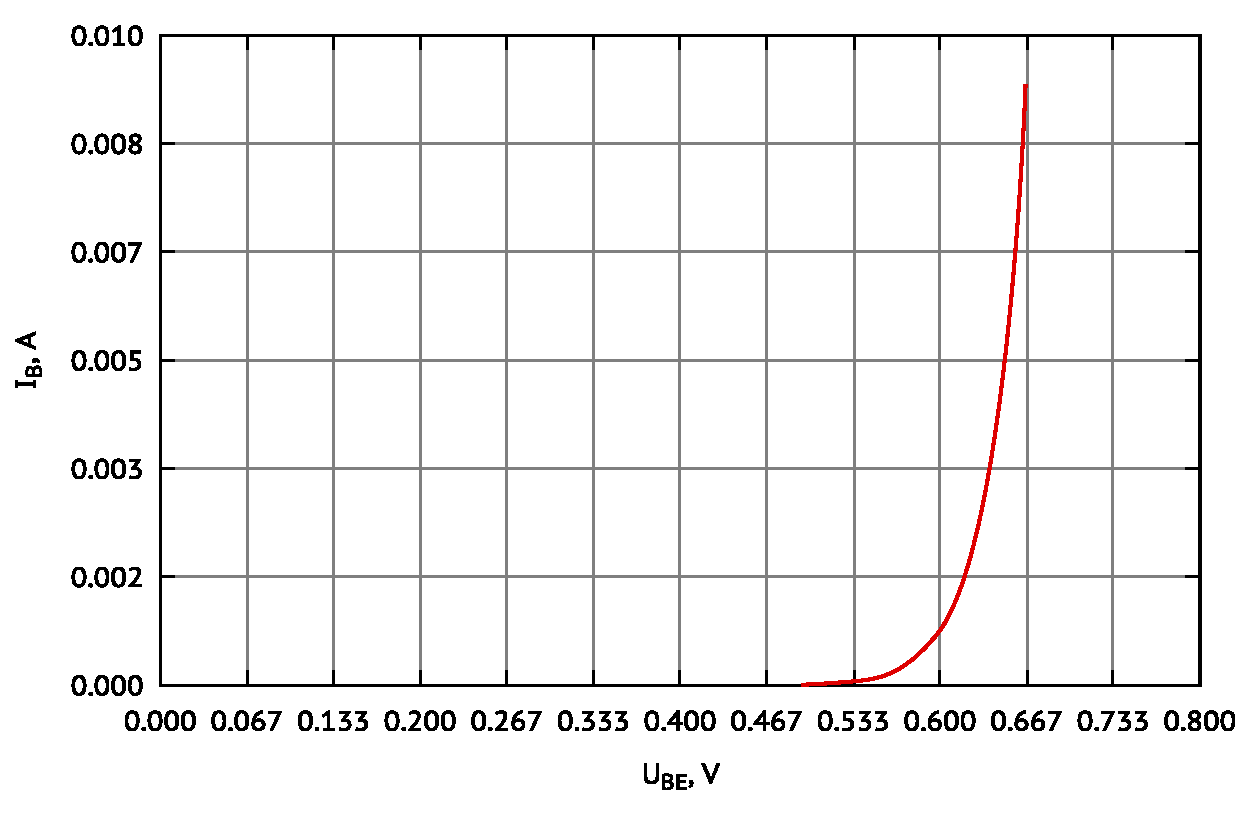
\includegraphics[width=0.45\textheight]{graph002-0.pdf}
					\caption{Третя отримана вхідна вольт-амперна характеристика}
					\label{fig:graph003}
				\end{figure}
				
		\subsection{Побудова вихідних вольт-амперних характеристик}
			%\subsubsection{Підготовка}
			%	Переводимо перемикач $SA2$ у потрібне положення, змінюємо налаштування осцилографа для значень вихідних вольт-амперних характеристик.
			\subsubsection{Побудова першої вольт-амперної характеристики}
				За допомогою осцилографа отримуємо першу вихідну вольт-амперну характеристику, зображену на рис. \ref{fig:graph004}.
				
				\begin{figure}[h]
					\centering
					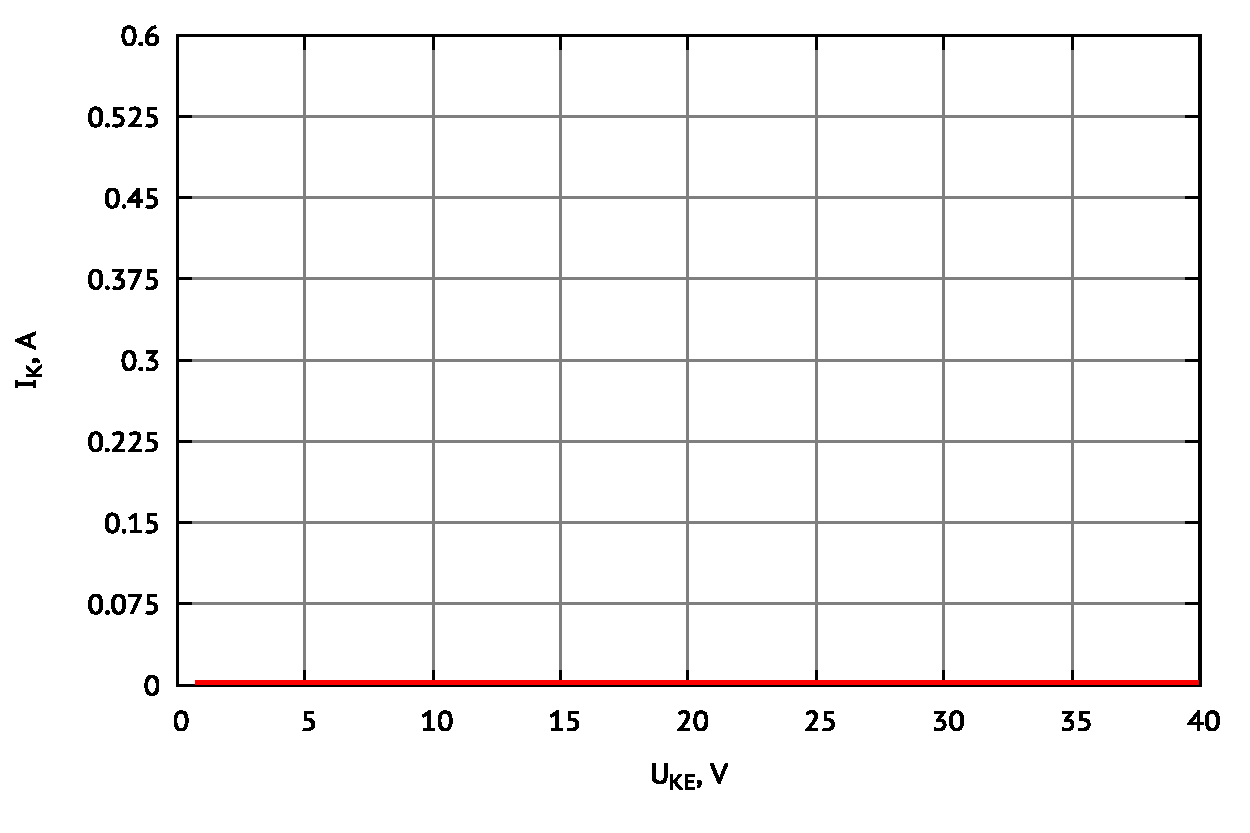
\includegraphics[width=0.45\textheight]{graph004.pdf}
					\caption{Перша отримана вихідна вольт-амперна характеристика}
					\label{fig:graph004}
				\end{figure}
				
			\subsubsection{Побудова другої вольт-амперної характеристики}
				За допомогою осцилографа отримуємо другу вихідну вольт-амперну характеристику, зображену на рис. \ref{fig:graph005}.
				
				\begin{figure}[h]
					\centering
					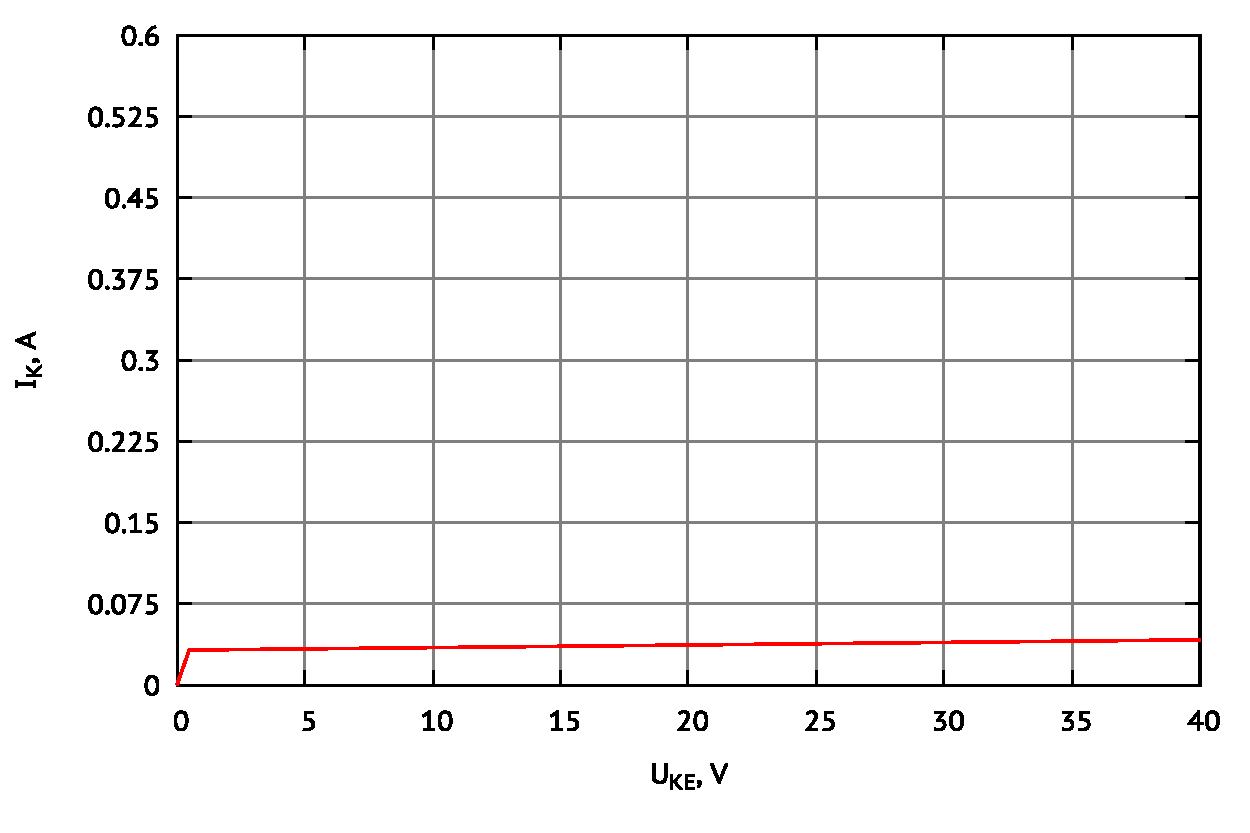
\includegraphics[width=0.45\textheight]{graph005.pdf}
					\caption{Друга отримана вихідна вольт-амперна характеристика}
					\label{fig:graph005}
				\end{figure}
				
			\subsubsection{Побудова третьої вольт-амперної характеристики}
				За допомогою осцилографа отримуємо третю вихідну вольт-амперну характеристику, зображену на рис. \ref{fig:graph005}.
				
				\begin{figure}[h]
					\centering
					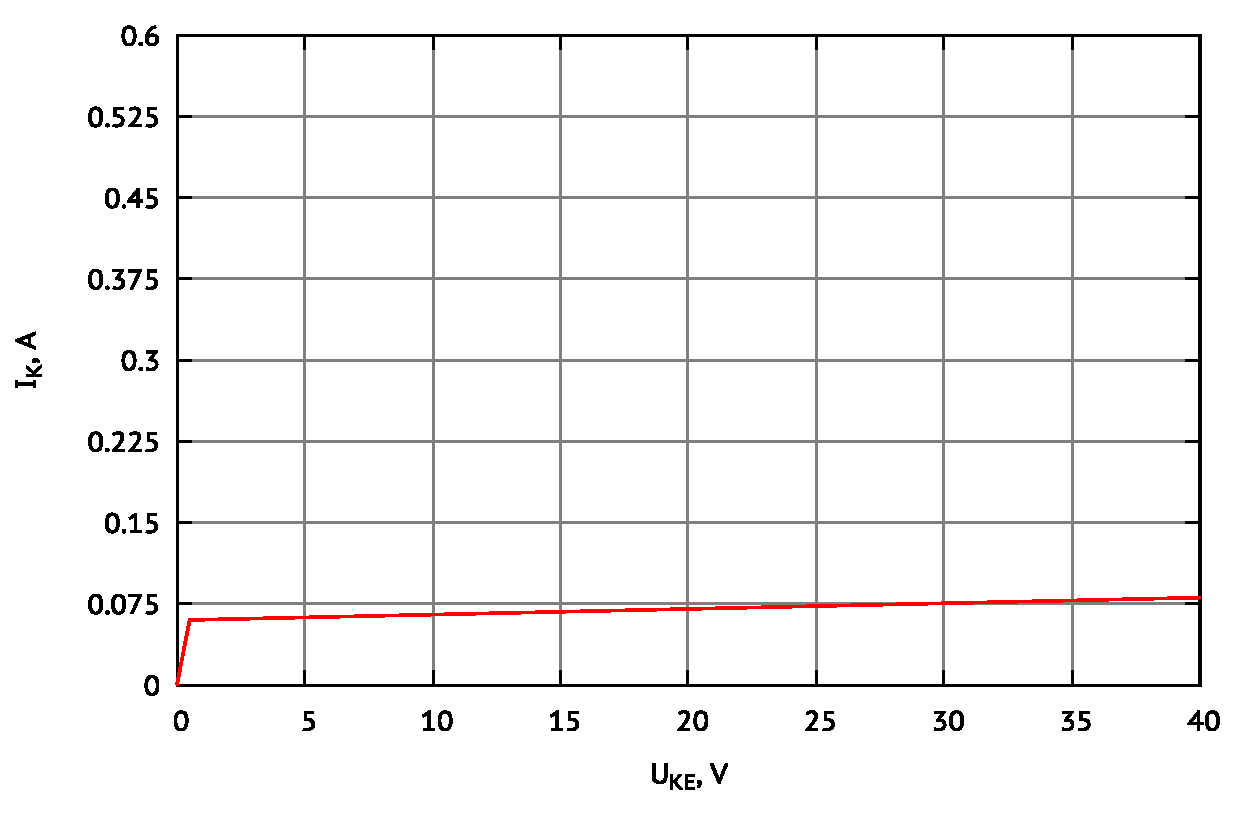
\includegraphics[width=0.45\textheight]{graph006.pdf}
					\caption{Третя отримана вихідна вольт-амперна характеристика}
					\label{fig:graph006}
				\end{figure}
				
	\section{Висновки}
		Виконуючи дану лабораторну роботу, ми:
			\begin{enumerate}
				\item Ознайомились з принципом дії, схемами ввімкнення і вольт-амперними характеристиками біполярного транзистора.
				\item Набули практичних навичок з побудови вольт-амперних характеристик.
				\item Вивчили схеми ввімкнення біполярних транзисторів і їх вольт-амперні характеристики. 
				\item Освоїли методику побудови за вхідною напругою інших струмів і напруг біполярного транзистора.
			\end{enumerate}
			
		Виконавши дослідження роботи біполярного транзистора у статичному режимі, ми переконались, що при напрузі $U_{\textnormal{КЕ}} = 0$ вхідна вольт-амперна характеристика дійсно починається на почтку координат. Крім того, ми удостовірились, що при збільшенні $U_{\textnormal{КЕ}}$ ($U_{\textnormal{КЕ}} > 0$) вхідна вольт-амперна характеристика зміщується вправо та вниз.
%			\begin{figure}[h!]
%			\centering
%				\begin{subfigure}[b]{0.3\textwidth}
%					\centering
%					\begin{circuitikz}
%						\draw
%						(0,0) node[above=2mm]{$-$}
%						to[short, *-*] (2,0)
%						to node[rground]{} (2, -1)
%						to[short, -*] (2,0)
%						to[short,*-*] node[above=2mm]{$UЕБ$} (4,0)
%						
%						(2,2) node[npn,rotate=90] (npn) {}
%						(2,0) to[short,*-] (npn.B)
%						
%						(0,2) node[above=2mm]{$К+$} to[short,*-] (npn.C)
%						(4,2) to[short,*-] (npn.E);
%					\end{circuitikz}
%				\end{subfigure}
%				\quad
%				\begin{subfigure}[b]{0.3\textwidth}
%				\end{subfigure}
%				\quad
%				\begin{subfigure}[b]{0.3\textwidth}
%				\end{subfigure}
%				\quad
%			\end{figure}
\end{document}